\begin{table*}[t!]
\begin{center}
\fontsize{10pt}{10.5pt}\selectfont
\setlength{\tabcolsep}{1mm}{
\begin{tabular}{l cc cc cc cc | cc}
\toprule
\multirow{2.5}{*}{\textbf{Method}} & \multicolumn{2}{c}{\textbf{2Wiki.}} & \multicolumn{2}{c}{\textbf{HotpotQA}} & \multicolumn{2}{c}{\textbf{MuSiQue}} & \multicolumn{2}{c}{\textbf{NQ}} & \multicolumn{2}{c}{\textbf{Avg.}} \\
\cmidrule(lr){2-3} \cmidrule(lr){4-5} \cmidrule(lr){6-7} \cmidrule(lr){8-9} \cmidrule(lr){10-11} 
 & \textbf{EM} & \textbf{F1} & \textbf{EM} & \textbf{F1} & \textbf{EM} & \textbf{F1} & \textbf{EM} & \textbf{F1} & \textbf{EM} & \textbf{F1} \\
\midrule
\multicolumn{11}{l}{\textbf{\textit{Qwen2.5-3B-Instruct}}} \\
\raisebox{-0.22\height}{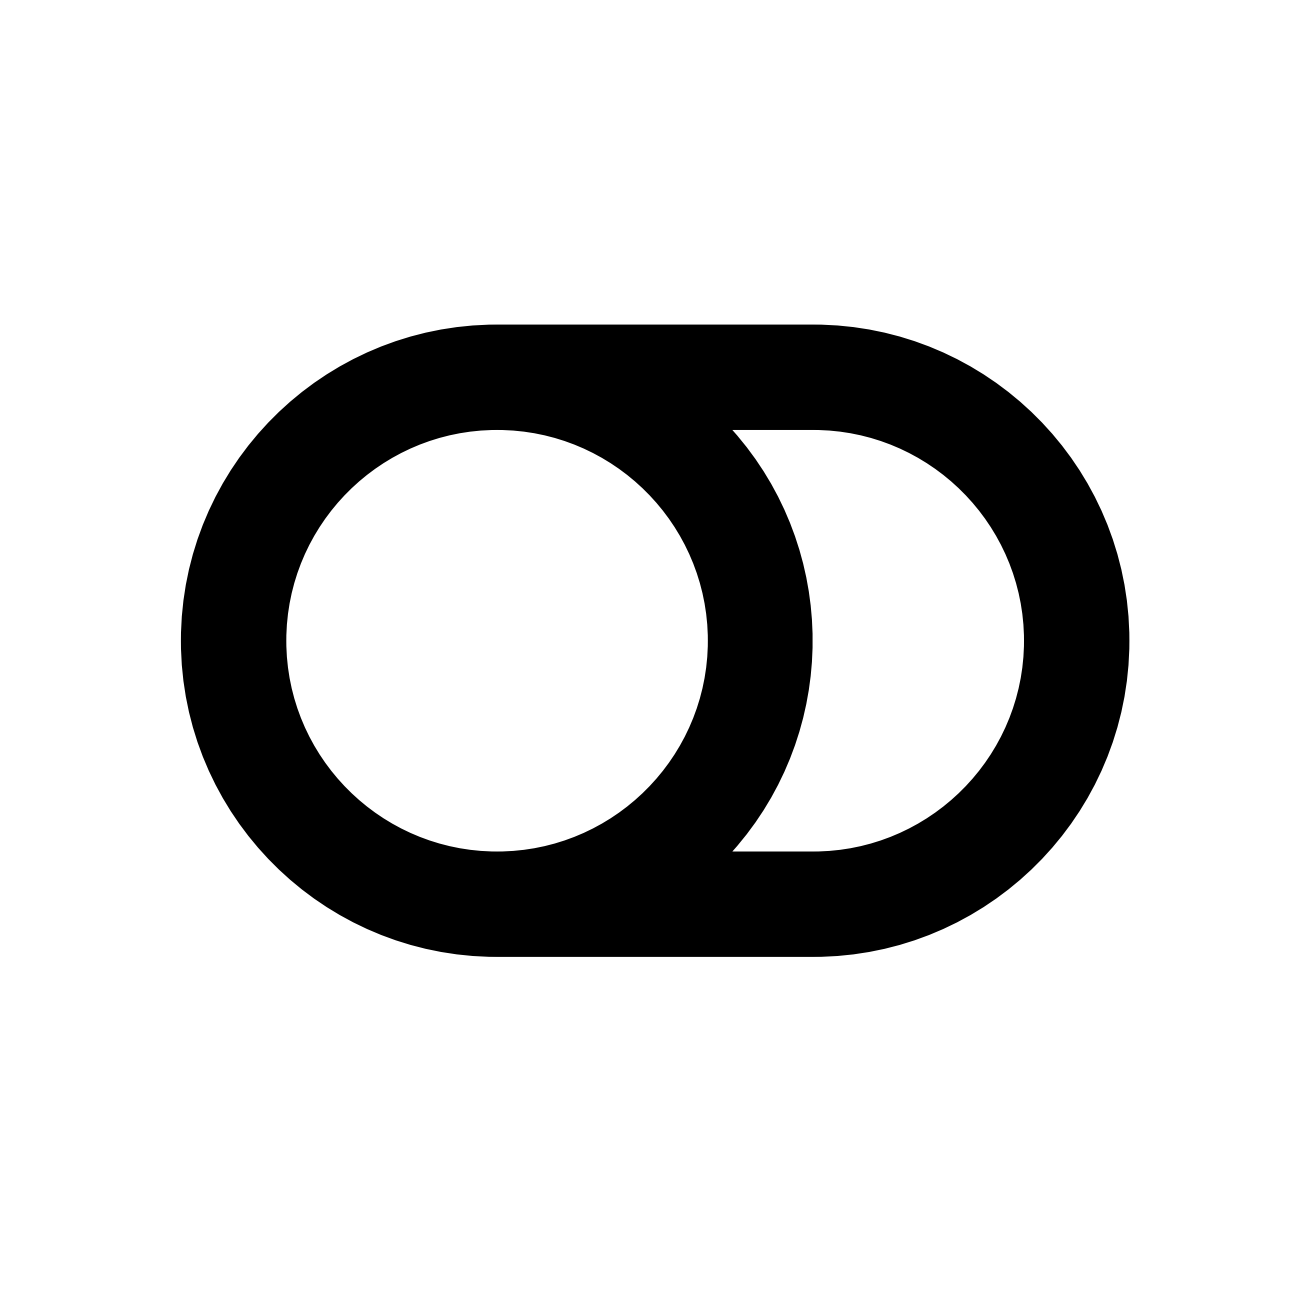
\includegraphics[width=0.02\textwidth]{Figures/close.png}}\raisebox{-0.22\height}{
\includegraphics[width=0.02\textwidth]{Figures/none.png}} NaiveGeneration & 2.34 & 7.59 & 6.25 & 11.16 & 0.78 & 3.67 & 2.34 & 8.90 & 2.93 & 7.83 \\
\raisebox{-0.22\height}{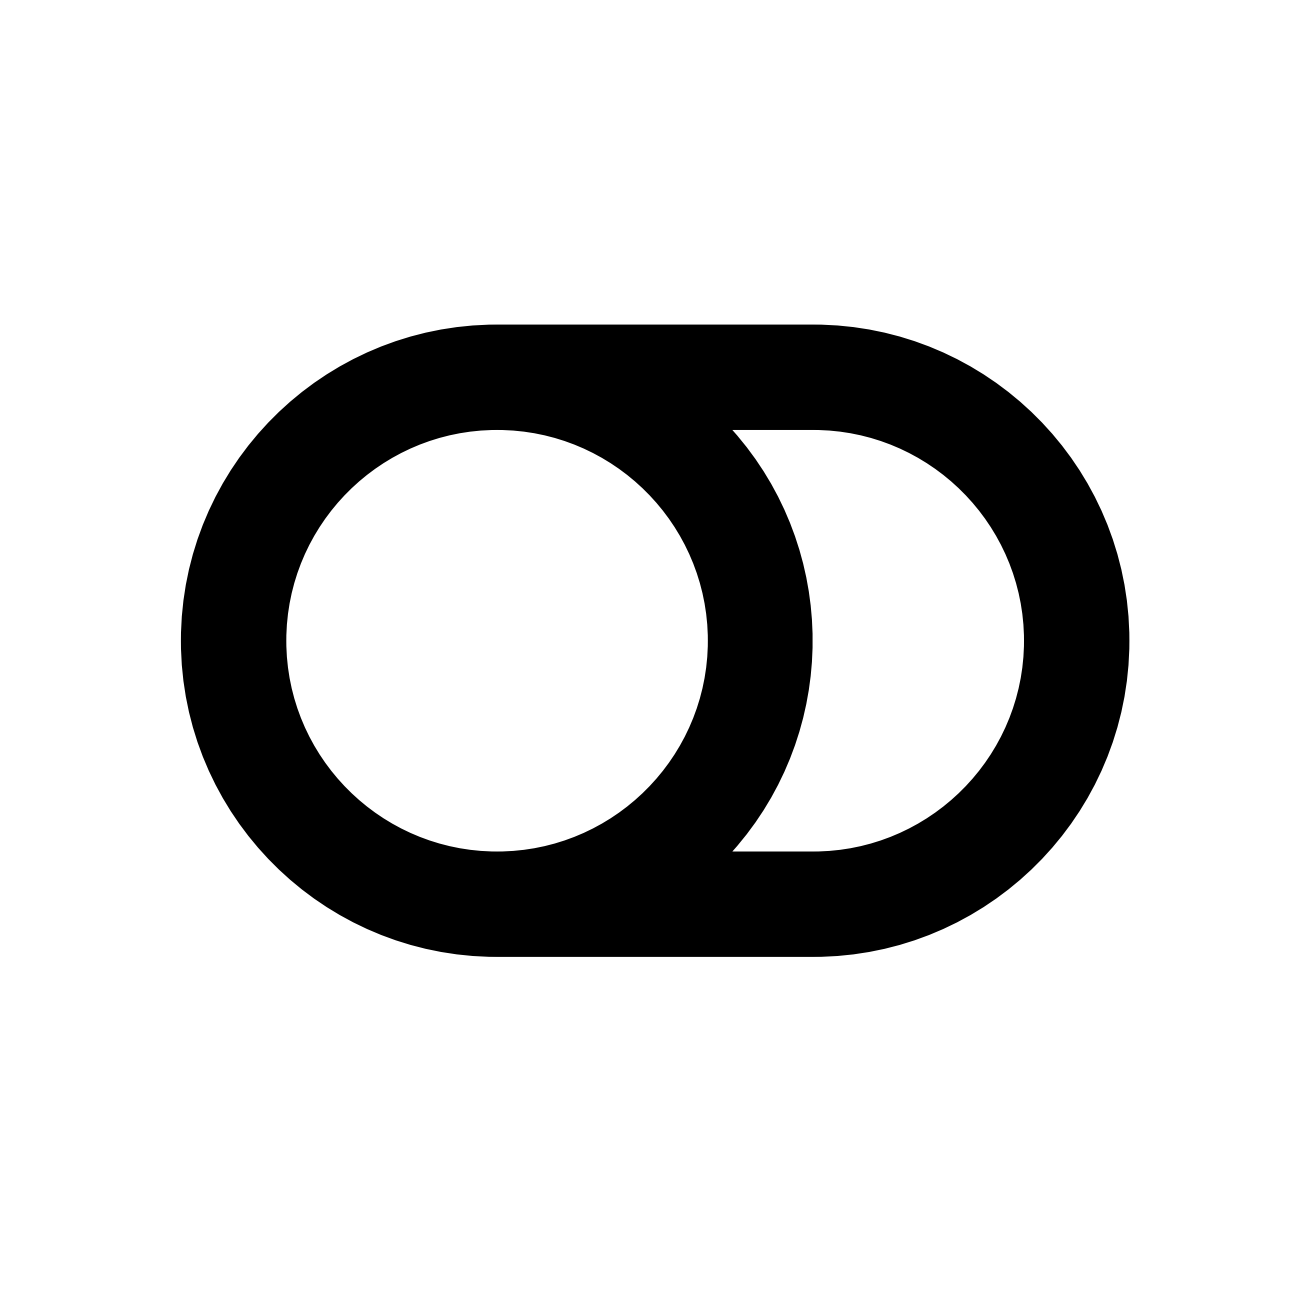
\includegraphics[width=0.02\textwidth]{Figures/close.png}}\raisebox{-0.22\height}{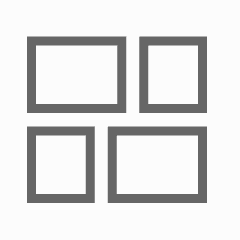
\includegraphics[width=0.02\textwidth]{Figures/chunk.png}} StandardRAG  & 3.91 & 12.52 & 7.03 & 15.41 & 0.00 & 2.92 & 0.00 & 10.69 & 2.74 & 10.39\\
\raisebox{-0.22\height}{
\includegraphics[width=0.02\textwidth]{Figures/open.png}}\raisebox{-0.22\height}{
\includegraphics[width=0.02\textwidth]{Figures/none.png}}SFT  & 7.03 & 12.40 & 10.94 & 16.48 & 1.56 & 5.04 & 3.12 & 11.23 & 5.66 & 11.29 \\
\raisebox{-0.22\height}{
\includegraphics[width=0.02\textwidth]{Figures/open.png}}\raisebox{-0.22\height}{
\includegraphics[width=0.02\textwidth]{Figures/none.png}} R1  & 20.31 & 28.45 & 20.31 & 25.33 & 3.12 & 8.07 & 11.72 & 21.51 & 13.87 & 20.84\\
\raisebox{-0.22\height}{
\includegraphics[width=0.02\textwidth]{Figures/open.png}}\raisebox{-0.22\height}{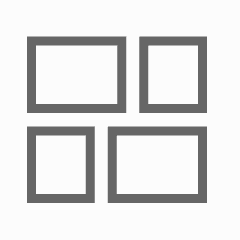
\includegraphics[width=0.02\textwidth]{Figures/chunk.png}} Search-R1  & 31.25 & 38.04 & 38.28 & 43.84 & 3.91 & 7.65 & 24.22 & 37.96 & 24.42 & 31.87 \\
\raisebox{-0.22\height}{
\includegraphics[width=0.02\textwidth]{Figures/open.png}}\raisebox{-0.22\height}{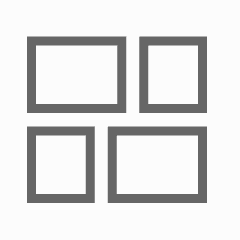
\includegraphics[width=0.02\textwidth]{Figures/chunk.png}} R1-Searcher  & 13.28 & 23.50 & 35.94 & 42.44 & 7.81 & 12.81 & 24.22 & 36.53 & 20.31 & 28.82 \\
\raisebox{-0.22\height}{
\includegraphics[width=0.02\textwidth]{Figures/open.png}}\raisebox{-0.22\height}{
\includegraphics[width=0.02\textwidth]{Figures/graph.png}} Graph-R1  & 50.00 & 57.56 & 50.78 & 56.75 & 32.81 & 40.51 & 30.47 & 44.75 & 41.02 & 49.89 \\
\midrule
\rowcolor{HyperGraphPro!15} \raisebox{-0.22\height}{
\includegraphics[width=0.02\textwidth]{Figures/open.png}}\raisebox{-0.22\height}{
\includegraphics[width=0.02\textwidth]{Figures/graph.png}} \textbf{HyperGraphPro} & \textbf{55.47} &\textbf{61.72} &\textbf{55.47} & \textbf{61.90} & \textbf{37.50} &\textbf{47.27} & \textbf{34.38} &\textbf{47.34} & \textbf{45.71}& \textbf{54.56}  \\
\midrule
\multicolumn{11}{l}{\textbf{\textit{Qwen2.5-7B-Instruct}}} \\
% \midrule
\raisebox{-0.22\height}{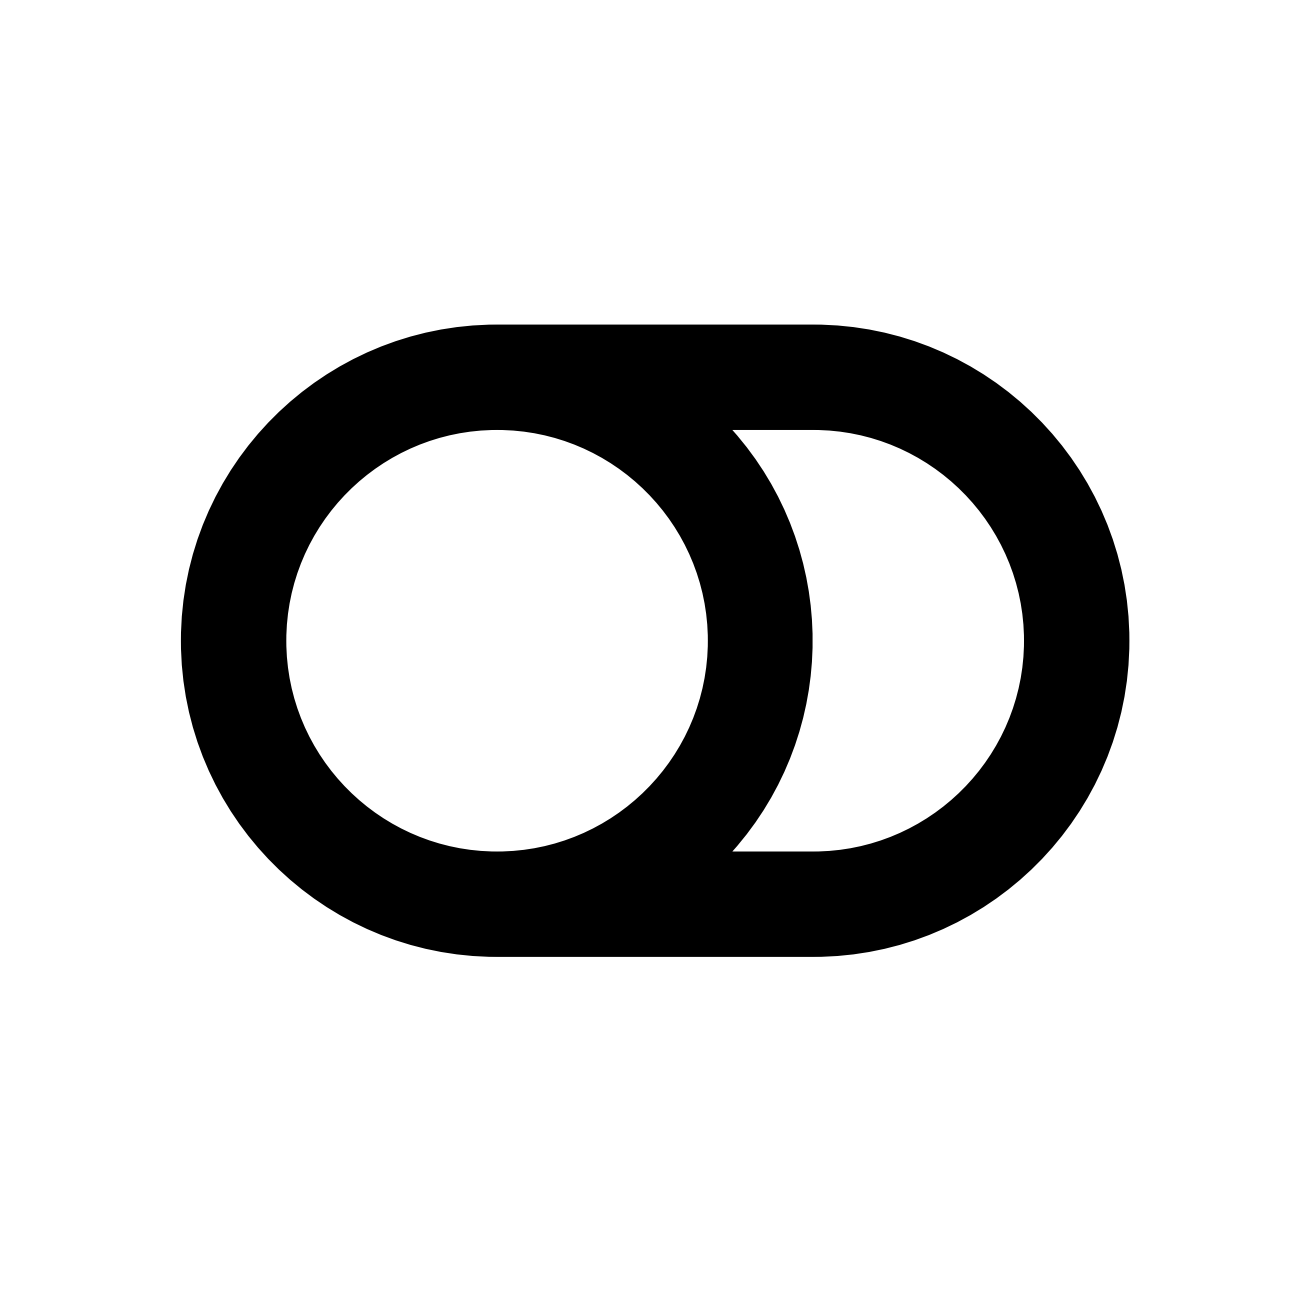
\includegraphics[width=0.02\textwidth]{Figures/close.png}}\raisebox{-0.22\height}{
\includegraphics[width=0.02\textwidth]{Figures/none.png}} NaiveGeneration  & 3.12 & 12.25 & 6.25 & 16.58 & 0.00 & 4.06 & 1.56 & 13.00 & 2.73 & 11.47 \\
\raisebox{-0.22\height}{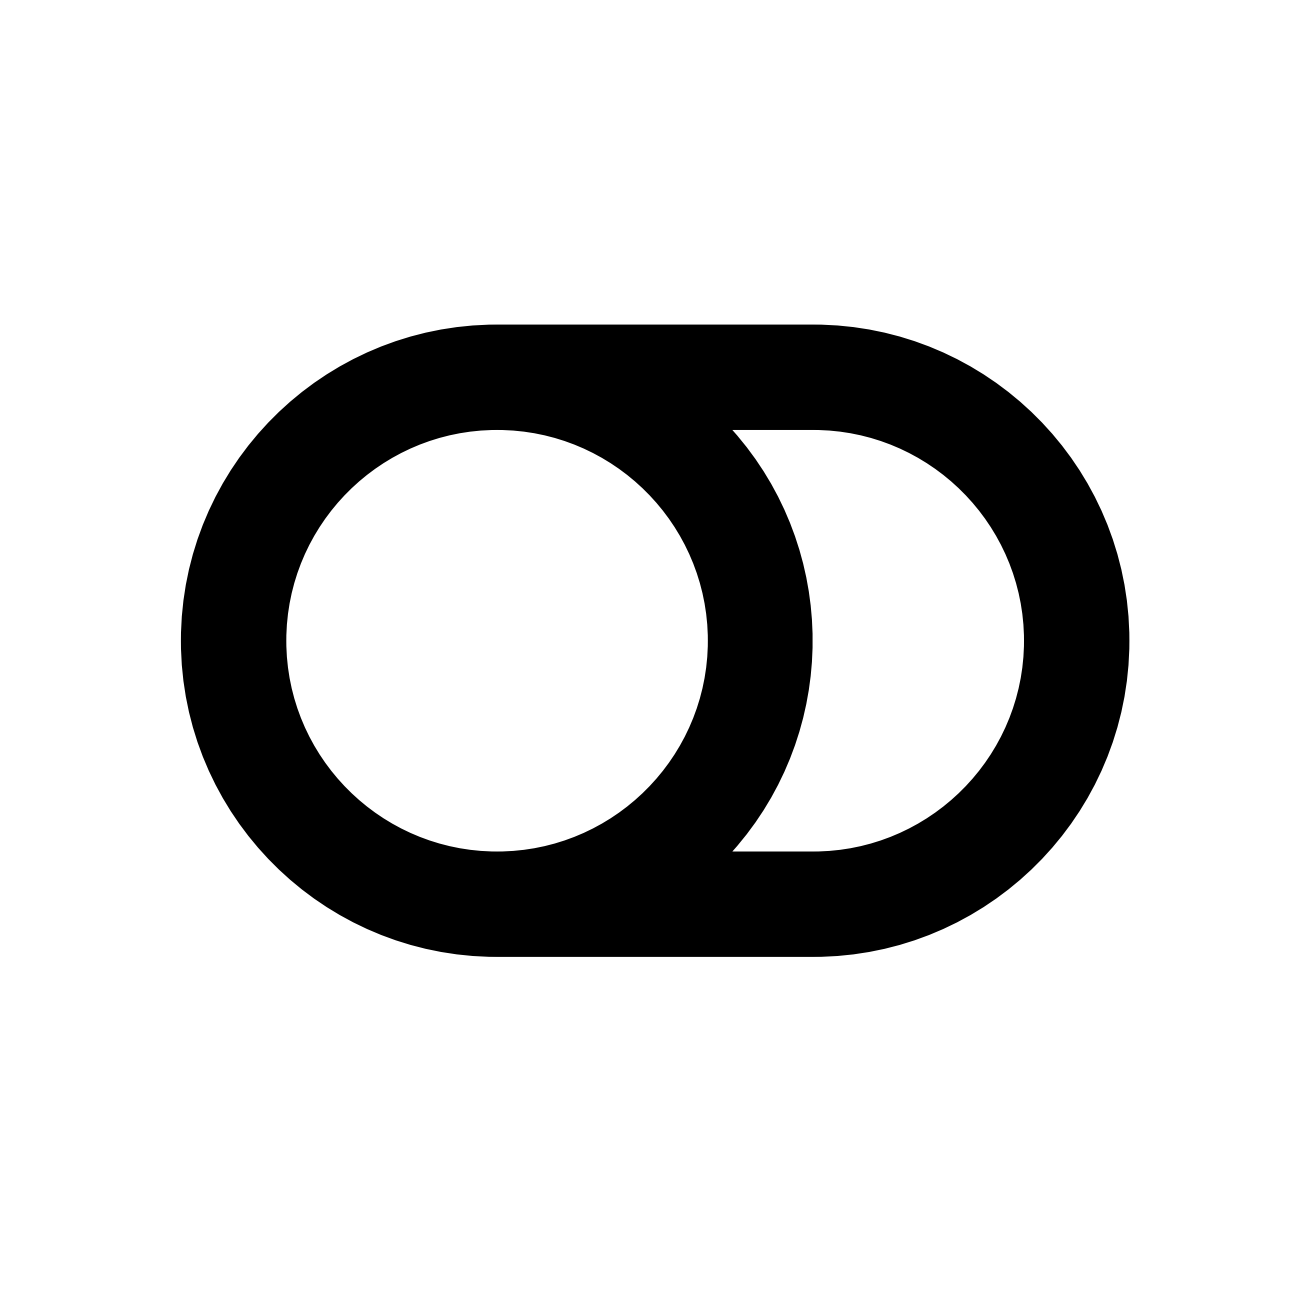
\includegraphics[width=0.02\textwidth]{Figures/close.png}}\raisebox{-0.22\height}{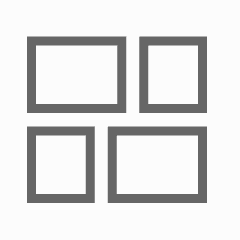
\includegraphics[width=0.02\textwidth]{Figures/chunk.png}} StandardRAG  & 7.81 & 12.75 & 10.16 & 21.10 & 0.78 & 4.53 & 1.56 & 15.97 & 5.08 & 13.59 \\
\raisebox{-0.22\height}{
\includegraphics[width=0.02\textwidth]{Figures/open.png}}\raisebox{-0.22\height}{
\includegraphics[width=0.02\textwidth]{Figures/none.png}}SFT  & 11.72 & 20.28 & 19.53 & 27.59 & 5.47 & 10.02 & 5.12 & 19.02 & 10.46 & 19.23 \\
\raisebox{-0.22\height}{
\includegraphics[width=0.02\textwidth]{Figures/open.png}}\raisebox{-0.22\height}{
\includegraphics[width=0.02\textwidth]{Figures/none.png}}  R1  & 25.00 & 30.99 & 31.25 & 37.05 & 7.03 & 14.53 & 16.41 & 28.45 & 19.92 & 27.76 \\
\raisebox{-0.22\height}{
\includegraphics[width=0.02\textwidth]{Figures/open.png}}\raisebox{-0.22\height}{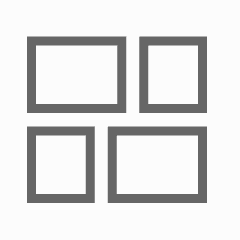
\includegraphics[width=0.02\textwidth]{Figures/chunk.png}} Search-R1  & 36.72 & 41.29 & 44.53 & 50.85 & 14.84 & 22.35 & 32.03 & 45.88 & 32.03 & 40.09 \\
\raisebox{-0.22\height}{
\includegraphics[width=0.02\textwidth]{Figures/open.png}}\raisebox{-0.22\height}{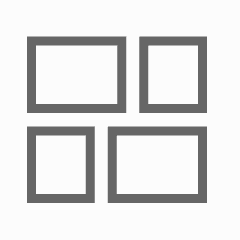
\includegraphics[width=0.02\textwidth]{Figures/chunk.png}} R1-Searcher  & 27.34 & 33.96 & 39.84 & 46.36 & 10.16 & 16.63 & 32.03 & 44.93 & 27.34 & 35.47 \\
\raisebox{-0.22\height}{
\includegraphics[width=0.02\textwidth]{Figures/open.png}}\raisebox{-0.22\height}{
\includegraphics[width=0.02\textwidth]{Figures/graph.png}} Graph-R1  & 55.47 & 65.04 & 57.03 & 62.69 & 36.72 & 46.17 & {33.59} & 49.87 & 45.70 & 55.94 \\
\midrule
\rowcolor{HyperGraphPro!15}\raisebox{-0.22\height}{
\includegraphics[width=0.02\textwidth]{Figures/open.png}}\raisebox{-0.22\height}{
\includegraphics[width=0.02\textwidth]{Figures/graph.png}} \textbf{HyperGraphPro} & \textbf{59.38}& \textbf{69.75} &\textbf{60.94} & \textbf{67.57} &\textbf{39.84} & \textbf{49.47} & \textbf{35.94}&\textbf{50.71} & \textbf{49.03} & \textbf{59.38} \\
\bottomrule
\end{tabular}%
}
\end{center}
\vspace{-10pt}
\caption{
Main results with best in \textbf{bold}. \raisebox{-0.5mm}{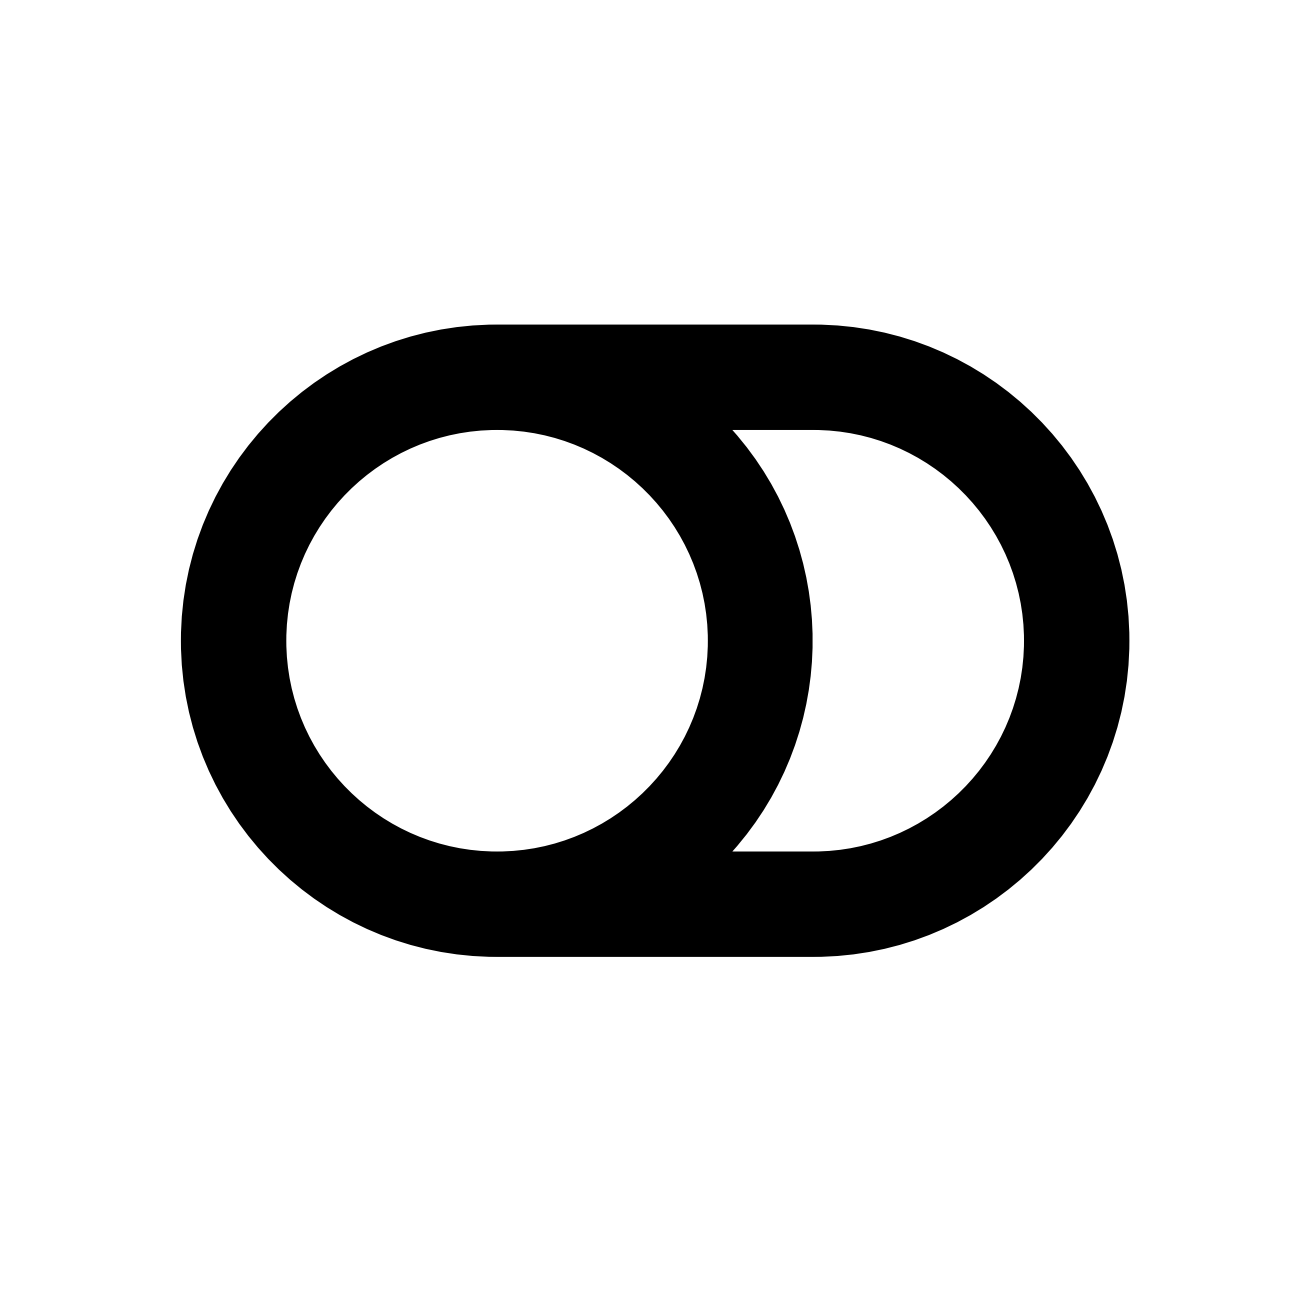
\includegraphics[width=0.02\textwidth]{Figures/close.png}} means prompt engineering, \raisebox{-0.5mm}{
\includegraphics[width=0.02\textwidth]{Figures/open.png}} means training, \raisebox{-0.5mm}{
\includegraphics[width=0.02\textwidth]{Figures/none.png}} means no knowledge interaction, \raisebox{-0.5mm}{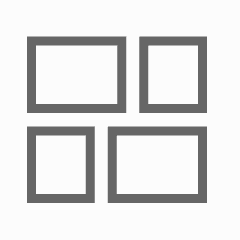
\includegraphics[width=0.02\textwidth]{Figures/chunk.png}} means chunk-based knowledge, and \raisebox{-0.5mm}{
\includegraphics[width=0.02\textwidth]{Figures/graph.png}} means graph-based knowledge.}
\label{T2}
\vspace{-12pt}
\end{table*}
